\documentclass[12pt,a4paper,titlepage]{article}
\usepackage{longtable,geometry}
\geometry{dvips,a4paper,margin=1.5in}

\usepackage[french]{babel}
\usepackage[utf8]{inputenc}
\usepackage[T1]{fontenc}

\usepackage{eurosym}

\usepackage[babel]{csquotes}
\MakeAutoQuote{«}{»}

\usepackage{graphicx}
\graphicspath{ {./images/} }

\usepackage{wrapfig}
\usepackage{caption}

\DeclareCaptionLabelFormat{simpleNumber}{#2}

\usepackage[final]{pdfpages}

\usepackage{rotating}
\usepackage{rotfloat}
\usepackage{float}

\usepackage{longtable, tabu}

\usepackage{makeidx}

\usepackage{verbatim}

\usepackage{blindtext}
\usepackage{scrextend}
\usepackage[pdfpagelabels, plainpages=false]{hyperref}
\usepackage[figure]{hypcap}

\setcounter{tocdepth}{3}

\usepackage[backend=biber]{biblatex}
\addbibresource{bibliography.bib}


\usepackage[toc,acronym,xindy]{glossaries}
\makeglossaries
\makeindex

\usepackage{xparse}

\DeclareDocumentCommand{\newdualentry}{ O{} O{} m m m m } {
    \newglossaryentry{gls-#3}{name={#5},text={#5\glsadd{#3}},
        description={#6},#1
    }
    \makeglossaries
    \newacronym[see={[Glossaire:]{gls-#3}},#2]{#3}{#4}{#5\glsadd{gls-#3}}
}


\newdualentry{isc}
  {ISC}
  {Institut des Sciences Cognitives}
  {Un centre de recherche dépendant du \gls{CNRS} spécialisé dans la recherche autour du cerveau}

\newdualentry{CNIL}
  {CNIL}
  {Comission Nationale de l'Informatique et des Libertés}
  {Autorité administrative indépendante française chargée de veiller à ce que l’informatique soit au service du citoyen et qu’elle ne porte atteinte ni à l’identité humaine, ni aux droits de l’Homme, ni à la vie privée, ni aux libertés individuelles ou publiques}

\newdualentry{CNRS}
  {CNRS}
  {Centre National de la Recherche Scientifique}
  {Le centre de recherche scientifique civil français}

\newdualentry{SF}
  {SF}
  {science-fiction}
  {Genre narratif consistant à raconter des fictions reposant sur des progrés scientifiques et techniques obtenus dans un futur plus ou moins lointain}

\newdualentry{ecas}
  {ECAS}
  {Entrainement des capacités de Concentration et d'Attention en milieu Scolaire}
  {Le projet de jeu sérieux sur lequel est basé mon stage} 

\newglossaryentry{gabor} {
  name = gabor,
  description = {Stimuli visuel de bas niveau, réalisé en faisant varier la luminance par rapport au fond},
  plural = gabors
}

\newglossaryentry{Psychotoolbox}{
  name = Psychotoolbox,
  description = {Bibliothèque de fonctions pour \gls{Matlab} dédiée à destination de la recherche en neurocience et en vision}
}

\newglossaryentry{Matlab} {
  name = Matlab,
  description = {Langage de programmation destiné aux calculs numériques et utilisé dans la recherche}
}

\newglossaryentry{Kiupe} {
  name = Kiupe,
  description = {Studio de développement de jeux sérieux lyonnais partenaire du projet \gls{ecas}}
}

\begin{document}


\begin{titlepage}
\begin{center}

\title{\LARGE{Stage à l'Institut des Sciences Cognitives}}
\author{\textsc{Gomez} Gwendoline \\Master 2 Développement de jeux vidéos \\Année universitaire 2017/2018}
\date{\today}

\end{center}
\end{titlepage}

\ClearShipoutPicture
\newpage

\newpage

\section*{Remerciements}

\newpage

\tableofcontents
\newpage

\listoffigures
\newpage

\section*{Introduction}
\addcontentsline{toc}{section}{Introduction}

\newpage

\section{Présentation}

\subsection{L'Institut des Sciences Cognitives}

Mon stage se déroule à l'\gls{ISC} à Bron. L'institut regroupe deux départements : le département de neurosciences cognitives et le département du langage, cerveau et cognition.
Chaque département regroupe des équipes de chercheurs qui étudient le comportement du cerveau, notamment de son aspect cognitif. Leurs travaux peuvent aboutir sur des papiers de
recherche pouvant détailler des découvertes ou des nouveaux protocoles par exemple.

\subsection{L'équipe}

\newpage

%  PARTIE 2.1 L'ATTENTION

\section{Projet en cours}

\subsection{L'attention}

\paragraph{}L'équipe de \emph{Suliann Ben Hamed} étudie le fonctionnement de l'attention. Des hypothèses ont été faites par des chercheurs sur la manière dont elle se manifeste et
comment nous l'utilisons. Le cerveau reçoit en permanence une multitude d'informations de la part de son environnement que l'on appelle des \emph{stimuli}. Il n'est pas capable de
traiter tous ces stimuli dans la durée et doit donc se focaliser sur les informations les plus importantes. A l'heure du numérique, l'être humain a tendance à perdre sa capacité
d'attention dans la durée. En effet, les smartphones et leur notifications par exemple ont tendance à sortir leur propriétaire assez régulièrement de leur tâche en cours. Ce qui
entrainerait une chute de performance sur des taches qui nécessitent une attention prolongée.

\paragraph{}D'après nos observations, nous pensons que l'\emph{attention sélective} est à la base de toutes les autres. Elle agit comme un filtre qui se focalise sur ce qui nous
parait le plus important parmi les informations reçues. Elle peut filtrer les informations selon leur aspect spatial, visuel, auditif ... (image de gauche sur la figure 
\ref{AspectSelectiveAttention}). Par exemple, pour porter notre focalisation sur un élément visuel, notre attention va faire bouger nos yeux et placer l'élément en plein milieu de
notre champs de vision. Cela permet d'avoir des informations plus détaillées que si l'élément était à la périphérie du champs visuel (image de droite sur la figure
\ref{AspectSelectiveAttention}). En même temps, si l'élément est purement visuel, l'attention va filtrer les informations auditives pour devoir en traiter le moins possible.

\begin{figure}[h]
    \begin{center}
    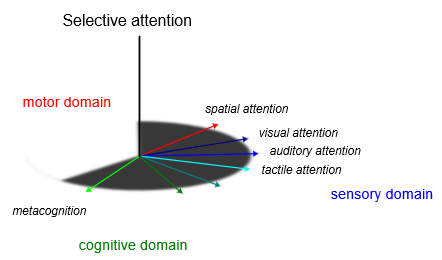
\includegraphics[width=12cm]{selectiveAttention.png}
    \end{center}
    \caption{Les différents aspects de l'attention sélective}
\label{AspectSelectiveAttention}
\end{figure}

\paragraph{}Nous pouvons observer une différence de capacités attentionnelles entre les personnes jeunes et âgées. En effet, les jeunes peuvent facilement déplacer leur attention
d'un élément à un autre et même sur plusieurs éléments à la fois. C'est \emph{l'attention divisive}. Elle permet, lors d'un cocktail par exemple, de pouvoir suivre plusieurs discussions
à la fois. En revanche, ils ont beaucoup de difficultés à maintenir leur attention efficacement dans le temps sur une tâche bien précise. Cette capacité s'appelle
\emph{l'attention soutenue} ou \emph{vigilance}. Les personnes plus âgées ont de par leur expérience une meilleure attention soutenue. Mais, du fait de leur âge, leur attention divise
n'est pas très performante.

\paragraph{}Notre capacité d'attention soutenue dépend de chacun. Plus la tâche est longue et moins il est facile de maintenir son attention. Si la tâche est prévisible, son exécution
va devenir un automatisme et augmentera le risque de vagabondage mental de la personne. Le \emph{vagabondage mental} est un état où la personne a des pensées qui n'ont aucun rapport
avec la tâche qu'elle exécute. Le moment où elle rentre dans l'état de vagabondage est appelé le \emph{décrochage} (voir figure \ref{SustainedAttention}).

\begin{figure}[h]
    \begin{center}
    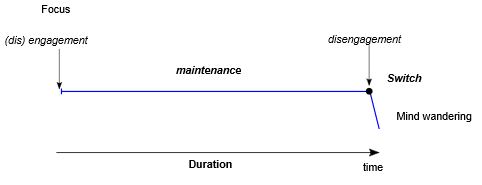
\includegraphics[width=12cm]{sustainedAttention.png}
    \end{center}
    \caption{L'évolution de la vigilance au cours du temps}
\label{SustainedAttention}
\end{figure}

\paragraph{}La difficulté de la tâche rentre aussi en jeu dans le décrochage d'une personne. En effet, si la tâche est trop facile, elle peut devenir prévisible, ennuyeuse et ne
pas nécessiter beaucoup de vigilance. Le sujet va alors vagabonder et est susceptible de rater un évènement important. Mais si celle-ci est trop difficile, elle va demander beaucoup
plus de vigilance et la personne peut décrocher de fatigue, de stress ... Pour de meilleurs performances, il faut également que le rapport effort de vigilance/motivation soit
intéressant. Si ces facteurs de difficulté et de motivation sont bien ajustés, la vigilance peut atteindre un optimum, symbolisant la capacité maximale de la personne (voir figure
\ref{DifficultyAndAttention}) , et qui diffère pour chacun. Cela va nous servir dans le paramétrage des tâches d'entrainement de l'attention dont nous parlerons dans la partie
\ref{TrainingSection}.

\begin{figure}[H]
    \begin{center}
    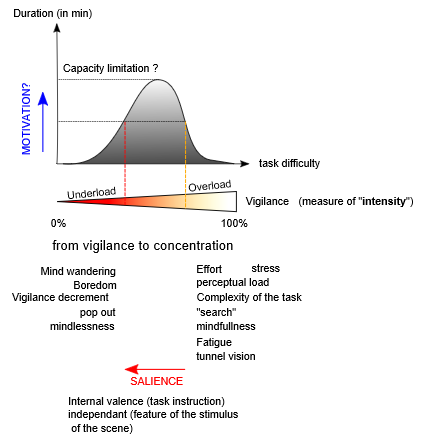
\includegraphics[width=10cm]{difficultyAndAttention.png}
    \end{center}
    \caption{Relation entre la difficulté de la tâche et la vigilance}
\label{DifficultyAndAttention}
\end{figure}

\paragraph{}Il existe une autre facette de l'attention. Celle-ci peut être sollicitée de la même manière tout au long d'une tâche qui ne change pas. Mais il est aussi possible que le
contexte change et que la réalisation de la tâche soit différente. C'est a dire que selon un contexte donné, une action peut être requise ou non. Il faut alors concentrer son
attention sur le fait de s'empêcher de faire cette action si le contexte le demande. On appelle cela l'\emph{attention exécutive}. Cet aspect nécessite un certain contrôle de notre
attention.


\paragraph{}Des études récentes sur des adolescents et des jeunes adultes ont montré un lien entre un usage non modéré des smartphones et surtout des applications de réseaux sociaux
comme Twitter, Facebook ... et une baisse des capacités d'attention soutenue \cite{ART01}. C'est pourquoi le projet \gls{ecas} a pour but d'utiliser ces supports censés perturber l'attention
pour l'améliorer grâce à un entrainement sous la forme d'un jeu sérieux.


%  PARTIE 2.2 L'ENTRAINEMENT


\newpage
\subsection{Les tâches d'entrainement}
\label{TrainingSection}

\paragraph{}L'amélioration d'une compétence nécessite de l'entrainement. C'est la même chose pour notre attention. Si l'on veut l'améliorer, il faut s'entrainer régulièrement.
L'entrainement de l'attention nécessite la répétition d'une tâche assez difficile pour nécessiter un peu plus que l'attention dont la personne est capable d'utiliser. Elle doit réussir
environ 75\% de la tache (entre 50 et 100\% sans jamais atteindre ces extrêmes) si elle veut s'améliorer.

\paragraph{}Lors de la réalisation d'une tâche, ce sur quoi notre attention doit se porter s'appelle \emph{la cible}. Tous les évènements autres pouvant nous tromper s'appellent
\emph{les distracteurs}. Deux tâches d'expérimentation ont été créées \emph{Simon Clavagnier} afin de vérifier certains points de l'entrainement et analyser les résultats. Ces tâches
ont été réalisée sous \gls{Matlab} avec la bibliothèque \gls{Psychotoolbox} .


\subsubsection{La tâche de CPT (Continuous Performance Task)}

\begin{wrapfigure}[7]{l}{2.3cm}
\vspace{-15pt}

\includegraphics[width=2.3cm]{gabor.jpg}
\captionsetup{labelformat=simpleNumber}
\caption{Gabor}
\end{wrapfigure}

\paragraph{Le dispositif}Le joueur est placé à une distance de 57 cm d'un écran grâce à une mentonnière qui permet de garder une certaine stabilité. Il dispose d'un clavier avec
lequel il se sert uniquement des touches \emph{espace} et \emph{1} et \emph{2} du pavé numérique. Des stimuli sous forme de \emph{\glspl{gabor}} sont présentés au sujet. La cible est un gabor
orienté à 45\degre. Les distracteurs sont des gabors dont l'orientation varie entre 6 et 42\degre par rapport à la cible. Les stimuli apparaissent aléatoirement pendant 80 ms. La
cible a une probabilité d'apparition de 12.5\%, soit $1/8$. Pour ne pas donner de rythme à l'apparition des stimuli, un temps d'attente de 200ms à 1 seconde les espace.

\begin{figure}[H]
    \begin{center}
    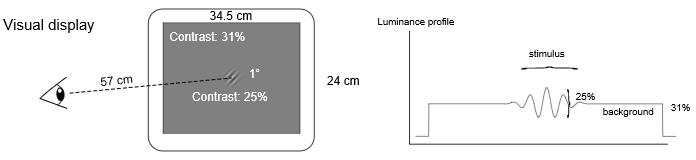
\includegraphics[width=13cm]{cptDispositif.png}
    \end{center}
    \caption{Dispositif de la tâche de CPT et modélisation d'un gabor}
\label{CptDispositif}
\end{figure}

\newpage
\paragraph{}Le sujet a pour objectif de taper sur la barre espace lorsqu'il reconnait la cible. Il dispose d'une seconde après l'apparition de la cible pour répondre. Nous ne cherchons
pas à mesurer les réflexes du sujet mais sa capacité de concentration. S'il trouve la cible, le sujet entend un bip. S'il tape sur un distracteur, il entend un cri. Le sujet a quatre
possibilités de réponses :
\begin{itemize}
\item Il appuie sur une cible. C'est une \textbf{\emph{détection correcte}} (\emph{hit}).
\item Il n'appuie pas sur un distracteur. C'est une \emph{rejection correct}.
\item Il appuie sur un distracteur. C'est une \textbf{\emph{fausse alarme}} (\emph{false alarm}).
\item Il n'appuie pas sur une cible. C'est une \textbf{\emph{omission}} (\emph{miss}).
\end{itemize}
Le sujet réalise plusieurs séries dans lesquelles il doit trouver la cible 80 fois. La durée complète de l'entrainement dépend des capacités du sujet. Elle oscille généralement entre
1 et 2h pour pouvoir observer des variations durant l'entrainement et des améliorations au fur et à mesure des sessions. Les séries sont entrecoupées d'un test de discrimination.

\begin{figure}[H]
    \begin{center}
    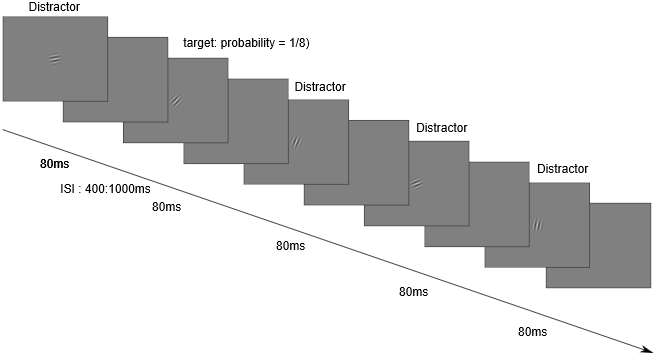
\includegraphics[width=13cm]{cptTask.png}
    \end{center}
    \caption{Exemple d'une partie de série de la tâche de CPT}
\label{CptTask}
\end{figure}

\paragraph{Le test de discrimination}Tout le monde n'a pas la même sensibilité visuelle. Il est donc nécessaire de déterminer le seuil de perception visuelle du sujet afin de calibrer
ses résultats en fonction. Le dispositif est le même que pour la tâche de CPT. La cible et les distracteurs sont les mêmes. On demande au sujet de fixer un point central et on affiche
des couples cible/distracteur présentées aléatoirement. Un premier stimulus est affiché pendant 80ms, suivi d'un masque pendant 50ms. Ce masque symbolise le gabor suivant dans la
tâche de CPT. Il augmente la difficulté car il empêche toute analyse du gabor postérieure à son apparition. Puis un écran vierge est présenté pendant 1 secondes. On affiche ensuite
le deuxième stimulus du couple de la même manière que le premier. Le sujet doit alors dire si la cible a été présentée en premier ou en deuxième avec les touches \emph{1} et \emph{2}
du pavé numérique. Il a 1.5 secondes pour répondre. Comme pour la tâche de CPT, s'il a juste, il entend un bip, sinon un cri. Les couples cibles/distracteurs peuvent apparaitre soit
au milieu de l'écran en vision centrale, soit légèrement décalé a droite ou a gauche, à la vision périphérique du sujet. Le test de discrimination dure environ 6 minutes, puis une
nouvelle série de la tâche de CPT est lancée.

\begin{figure}[H]
    \begin{center}
    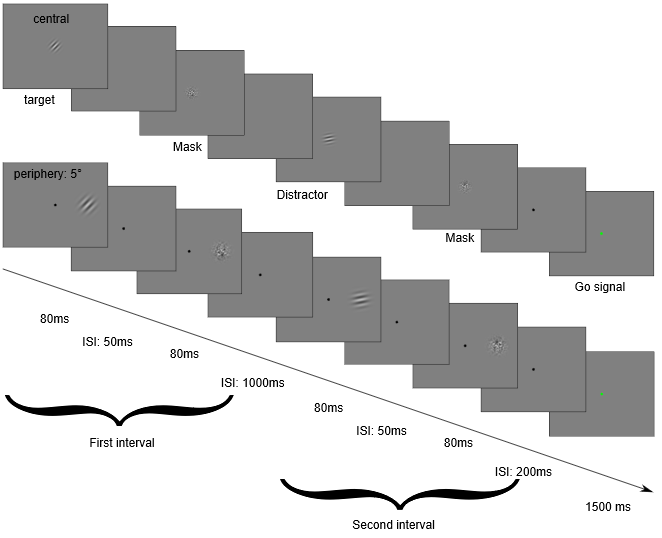
\includegraphics[width=13cm]{cptDiscriminationTask.png}
    \end{center}
    \caption{Exemple d'une partie de test de discrimination}
\label{CptDiscriminationTask}
\end{figure}


\paragraph{Traitement des données}Les données collectées sont propres à chaque sujet et sont analysées par session. On peut ainsi voir l'impact de l'entrainement sur le
sujet et comparer son évolution par rapport aux autres. J'ai pu participer à la tâche d'entrainement en tant que sujet afin de bien comprendre son fonctionnement. \`{A}
chaque session, mes performances se sont améliorées. La figure \ref{CptPerformance} représente mes résultats sur 5 sessions.

\begin{figure}[H]
    \begin{center}
    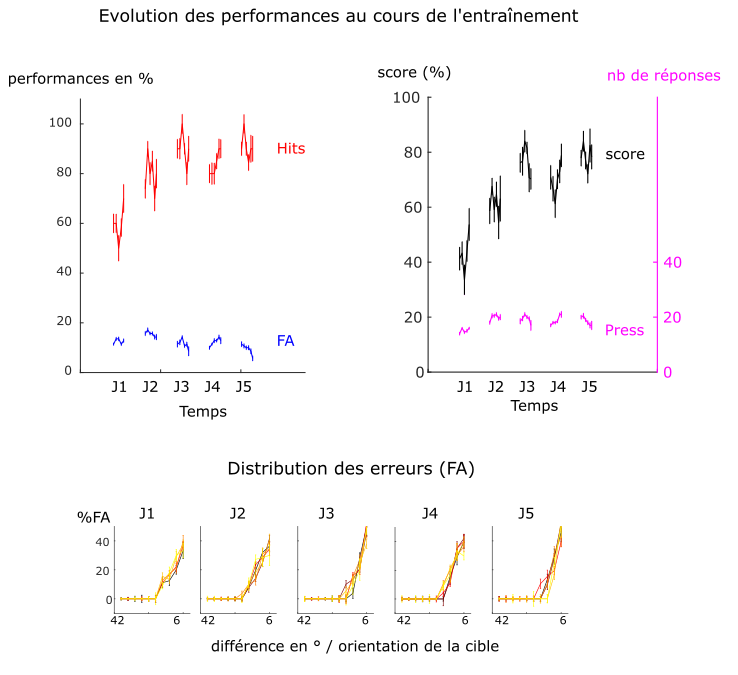
\includegraphics[width=10cm]{cptPerformance.png}
    \end{center}
    \caption{L'évolution de mes performances sur la tâche de CPT}
\label{CptPerformance}
\end{figure}

\paragraph{}Si on regarde le pourcentage de hits en rouges et celui du score en noir, on remarque qu'ils augmentent significativement au fur et à mesure des sessions. Le nombre de FA
au contraire est en baisse alors que le nombre de fois où la touche espace est pressée ne bouge pas beaucoup. On constate aussi que la distribution des erreurs, qui correspond aux
résultats du test de discrimination, ne bouge pas beaucoup. Cela veut dire que ce n'est pas ma capacité à reconnaitre la cible qui a changée mais plutôt mes capacités de concentration
et de contrôle sur mon attention.

 \newpage

\subsubsection{Le gaborium}

\paragraph{Le dispositif}Le gaborium utilise également des \glspl{gabor} comme stimulus. Un écran rempli d'une multitudes de gabors de tailles et d'orientations différentes est montré
au sujet. Tous les distracteurs sont des gabors avec une direction et une vitesse de mouvement constante. La cible est un gabor dont la direction et la vitesse changent constamment.
Dans cette tâche, le sujet doit cliquer sur la cible avec la souris des qu'il l'aperçoit. La cible disparaît alors et une autre cible fait son apparition après un laps de temps
variable. L'œil droit du sujet est traqué à l'aide d'un eye tracker Eyelink. Il doit également appuyer sur la barre espace s'il sent qu'il n'est plus concentré sur la tâche de Gaborium.

\begin{figure}[H]
    \begin{center}
    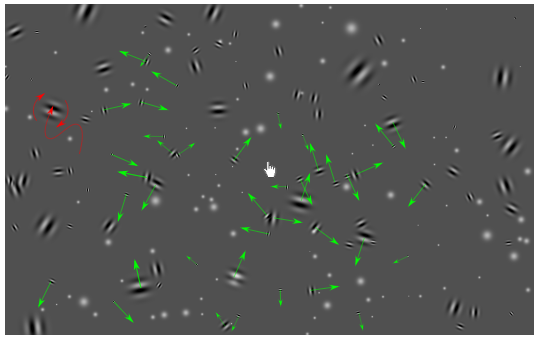
\includegraphics[width=13cm]{gaborium.png}
    \end{center}
    \caption{Gaborium avec les directions de certains gabors affichées}
\label{Gaborium}
\end{figure}

\paragraph{Traitement des données}\textcolor{red}{Il faut traiter les données mais on sait pas comment donc il faut demander à Simon !!!}


\newpage

\section{Problématique}

\paragraph{}D'après la recherche, il est possible d'améliorer son attention avec de l'entrainement. L'équipe de \emph{Suliann Ben Hamed} l'a prouvé à l'aide de protocoles expérimentaux
dont les résultats ont été très satisfaisants. Le but est maintenant de pouvoir tester ces protocoles en grandeur nature sur des élèves et d'observer leurs impacts sur leur
concentration en cours, voir même sur leurs résultats. Mais ces protocoles ont néanmoins un gros défaut. Ils ne sont pas attractifs et sont même rébarbatifs. Il est donc difficile de
motiver un élève a consacrer 1h par jour de son temps sur cet entrainement. C'est pourquoi l'objectif de mon stage est trouver un moyen de rendre ces entrainements attractifs, voir
même addictifs. L'idée est de réaliser un jeu vidéo qui ressemble plus ou moins aux protocoles mais qui aurait les mêmes effets. La question qui en découle est donc :
\begin{quote}
\textbf{Peut-on entrainer l'attention à l'aide d'un jeu vidéo ?}
\end{quote}

A cette questions s'ajoutent quelques difficultés à ne pas négliger, la première étant la communication avec les chercheurs. En effet, il est nécessaire de comprendre leurs
recherches afin de bien saisir leurs besoins et de parler "la même langue".

De plus, il est important de prendre en compte les contraintes techniques notamment en matière de réseau et de stockage de données permettant l'analyse des entrainements.


\newpage

\section{Réalisation}

\subsection{Etude du besoin}

\subsection{Mise en place de l'environnement}

\subsection{Prototypage du premier jeu}

\subsection{Gestion des données}

\newpage 

\section*{Conclusion}
\addcontentsline{toc}{section}{Conclusion}

\paragraph{}Le but de ce stage était la réalisation d'un jeu sérieux permettant d'entrainer l'attention en milieu scolaire de n'importe quel étudiant. Nous nous sommes inspirés des
tâches d'entrainement existantes afin de créer un prototype fonctionnel. Celui-ci permet grâce à sa modularité de jouer sur différents aspects de l'attention. Les données de chaque
joueur sont récupérées pour être analysées. Le prochain objectif est de diffuser ce prototype et d'observer son impact sur l'évolution des capacités attentionnelles des joueurs.

\paragraph{}Ce stage a été formateur pour moi pour plusieurs raisons. Il y a tout d'abord le contexte du projet. Je suis très intéressée par les jeux sérieux et ce projet m'a permis de
comprendre les enjeux d'un jeu vidéo à la fois en milieu scolaire, mais aussi dans le cadre de la recherche. Ensuite, le projet en étant à ses débuts, nous avons participé au processus
de création du jeu dans sa globalité, de son concept jusqu'à l'obtention d'un prototype fonctionnel. Nous nous sommes heurtés à différentes problématiques, techniques et fonctionnelles,
que ce soit sur le fonctionnement du jeu ou la gestion des données.

\paragraph{}Ce projet m'ayant beaucoup plus, et ayant eu une proposition du Dr.\emph{Suliann Ben Hamed}, j'ai fait le choix de monter un dossier de thèse CIFRE pour pouvoir continuer de
travailler sur ce projet. Cette thèse se fera en collaboration avec l'entreprise Kiupe, partenaire du projet.

\newpage

\printglossary[type=\acronymtype]
\newpage

\printglossary
\newpage

\printbibliography[heading=bibintoc, title={Bibliographie}]

\section*{Annexes}
\addcontentsline{toc}{section}{Annexes}

\newpage

\begin{abstract}

\paragraph{}Un constat des professeurs a été fait concernant la difficulté de leurs élèves à se concentrer sur leurs cours. Une solution possible est de proposer aux étudiants un
entrainement leur permettant d'améliorer leurs capacités d'attention pour pouvoir être plus attentifs en cours. Des outils existent déjà pour les enfants ayant des problèmes
attentionnels avérés, par exemple les hyperactifs, mais ces outils ne sont pas adaptés au reste de la population. Il était donc nécessaire de créer un nouvel outil. Pour être ludique
et attractif auprès de ce public, le choix a été fait de créer un jeu vidéo sérieux. Ce mémoire explique le processus de création de ce jeu réalisé dans le cadre de mon stage de fin
de Master 2 à l'\gls{isc}, depuis les premiers concepts de gameplay jusqu'à la réalisation d'un jeu fonctionnel.

\end{abstract}





\end{document}